
\documentclass{article}

\usepackage{fancyhdr} % Required for custom headers
\usepackage{lastpage} % Required to determine the last page for the footer
\usepackage{extramarks} % Required for headers and footers
\usepackage[usenames,dvipsnames]{color} % Required for custom colors
\usepackage{graphicx} % Required to insert images
\usepackage{listings} % Required for insertion of code
\usepackage{courier} % Required for the courier font
\usepackage{lipsum} % Used for inserting dummy 'Lorem ipsum' text into the template
\usepackage{caption}
\usepackage{subcaption}
\usepackage{amsmath}
\usepackage{systeme}

\graphicspath{ {../../../datasets/images/chapter_02/} }

% Margins
\topmargin=-0.45in
\evensidemargin=0in
\oddsidemargin=0in
\textwidth=6.5in
\textheight=9.0in
\headsep=0.25in

\linespread{1.1} % Line spacing

% Set up the header and footer
\pagestyle{fancy}
\lhead{\hmwkAuthorName} % Top left header
\chead{\hmwkClass\ (\hmwkClassInstructor\ \hmwkClassTime): \hmwkTitle} % Top center head
\rhead{\firstxmark} % Top right header
\lfoot{\lastxmark} % Bottom left footer
\cfoot{} % Bottom center footer
\rfoot{Page\ \thepage\ of\ \protect\pageref{LastPage}} % Bottom right footer
\renewcommand\headrulewidth{0.4pt} % Size of the header rule
\renewcommand\footrulewidth{0.4pt} % Size of the footer rule

\setlength\parindent{0pt} % Removes all indentation from paragraphs

%----------------------------------------------------------------------------------------
%	CODE INCLUSION CONFIGURATION
%----------------------------------------------------------------------------------------

\definecolor{MyDarkGreen}{rgb}{0.0,0.4,0.0} 
\lstloadlanguages{Matlab}
\lstset{language=Matlab,
        frame=single,
        basicstyle=\small\ttfamily,
        keywordstyle=[1]\color{Blue}\bf,
        keywordstyle=[2]\color{Purple},
        keywordstyle=[3]\color{Blue}\underbar,
        identifierstyle=,
        commentstyle=\usefont{T1}{pcr}{m}{sl}\color{MyDarkGreen}\small, 
        stringstyle=\color{Purple},
        showstringspaces=false,
        tabsize=5, 
        morekeywords={rand},
        morekeywords=[2]{on, off, interp},
        morekeywords=[3]{test},
        morecomment=[l][\color{Blue}]{...},
        numbers=left,
        firstnumber=1,
        numberstyle=\tiny\color{Blue},
        stepnumber=5
}

% Creates a new command to include a perl script, the first parameter is the filename of the script (without .pl), the second parameter is the caption
\newcommand{\matlabscript}[2]{
\begin{itemize}
\item[]\lstinputlisting[caption=#2,label=#1]{#1.m}
\end{itemize}
}

%----------------------------------------------------------------------------------------
%	DOCUMENT STRUCTURE COMMANDS
%	Skip this unless you know what you're doing
%----------------------------------------------------------------------------------------

% Header and footer for when a page split occurs within a problem environment
\newcommand{\enterProblemHeader}[1]{
\nobreak\extramarks{#1}{#1 continued on next page\ldots}\nobreak
\nobreak\extramarks{#1 (continued)}{#1 continued on next page\ldots}\nobreak
}

% Header and footer for when a page split occurs between problem environments
\newcommand{\exitProblemHeader}[1]{
\nobreak\extramarks{#1 (continued)}{#1 continued on next page\ldots}\nobreak
\nobreak\extramarks{#1}{}\nobreak
}

\setcounter{secnumdepth}{0} % Removes default section numbers
\newcounter{homeworkProblemCounter} % Creates a counter to keep track of the number of problems

\newcommand{\homeworkProblemName}{}
\newenvironment{homeworkProblem}[1][Problem \arabic{homeworkProblemCounter}]{ % Makes a new environment called homeworkProblem which takes 1 argument (custom name) but the default is "Problem #"
\stepcounter{homeworkProblemCounter} % Increase counter for number of problems
\renewcommand{\homeworkProblemName}{#1} % Assign \homeworkProblemName the name of the problem
\section{\homeworkProblemName} % Make a section in the document with the custom problem count
\enterProblemHeader{\homeworkProblemName} % Header and footer within the environment
}{
\exitProblemHeader{\homeworkProblemName} % Header and footer after the environment
}

\newcommand{\problemAnswer}[1]{ % Defines the problem answer command with the content as the only argument
\noindent\framebox[\columnwidth][c]{\begin{minipage}{0.98\columnwidth}#1\end{minipage}} % Makes the box around the problem answer and puts the content inside
}

\newcommand{\homeworkSectionName}{}
\newenvironment{homeworkSection}[1]{ % New environment for sections within homework problems, takes 1 argument - the name of the section
\renewcommand{\homeworkSectionName}{#1} % Assign \homeworkSectionName to the name of the section from the environment argument
\subsection{\homeworkSectionName} % Make a subsection with the custom name of the subsection
\enterProblemHeader{\homeworkProblemName\ [\homeworkSectionName]} % Header and footer within the environment
}{
\enterProblemHeader{\homeworkProblemName} % Header and footer after the environment
}

%----------------------------------------------------------------------------------------
%	NAME AND CLASS SECTION
%----------------------------------------------------------------------------------------

\newcommand{\hmwkTitle}{Assignment\ \#1}
\newcommand{\hmwkDueDate}{Monday,\ March\ 26,\ 2018}
\newcommand{\hmwkClass}{IMAGE\ PROCESSING} % Course/class
\newcommand{\hmwkClassTime}{14:00pm} % Class/lecture time
\newcommand{\hmwkClassInstructor}{gslee} % Teacher/lecturer
\newcommand{\hmwkAuthorName}{Tien Anh Nguyen} % Your name

%----------------------------------------------------------------------------------------
%	TITLE PAGE
%----------------------------------------------------------------------------------------

\title{
\vspace{2in}
\textmd{\textbf{\hmwkClass:\ \hmwkTitle}}\\
\normalsize\vspace{0.1in}\small{Due\ on\ \hmwkDueDate}\\
\vspace{0.1in}\large{\textit{\hmwkClassInstructor\ \hmwkClassTime}}
\vspace{3in}
}

\author{\textbf{\hmwkAuthorName}}
\date{} % Insert date here if you want it to appear below your name

%----------------------------------------------------------------------------------------

\begin{document}

\maketitle

%----------------------------------------------------------------------------------------
%	TABLE OF CONTENTS
%----------------------------------------------------------------------------------------

%\setcounter{tocdepth}{1} % Uncomment this line if you don't want subsections listed in the ToC

\newpage
\tableofcontents
\newpage

%----------------------------------------------------------------------------------------
%	PROBLEM 1
%----------------------------------------------------------------------------------------

% To have just one problem per page, simply put a \clearpage after each problem

\begin{homeworkProblem}
\subsection{Vanishing Line}
\matlabscript{problem_1}{Problem 1 demonstration in Matlab}

In the Cartesian coordinate system, given 2 parallel lines:
$L_1$ is $x - 2y + 5 = 0$ and $L_2$ is $x - 2y + 1 = 0$

\begin{figure}[h]
	\begin{subfigure}[t]{0.3\textwidth}
		\centering
		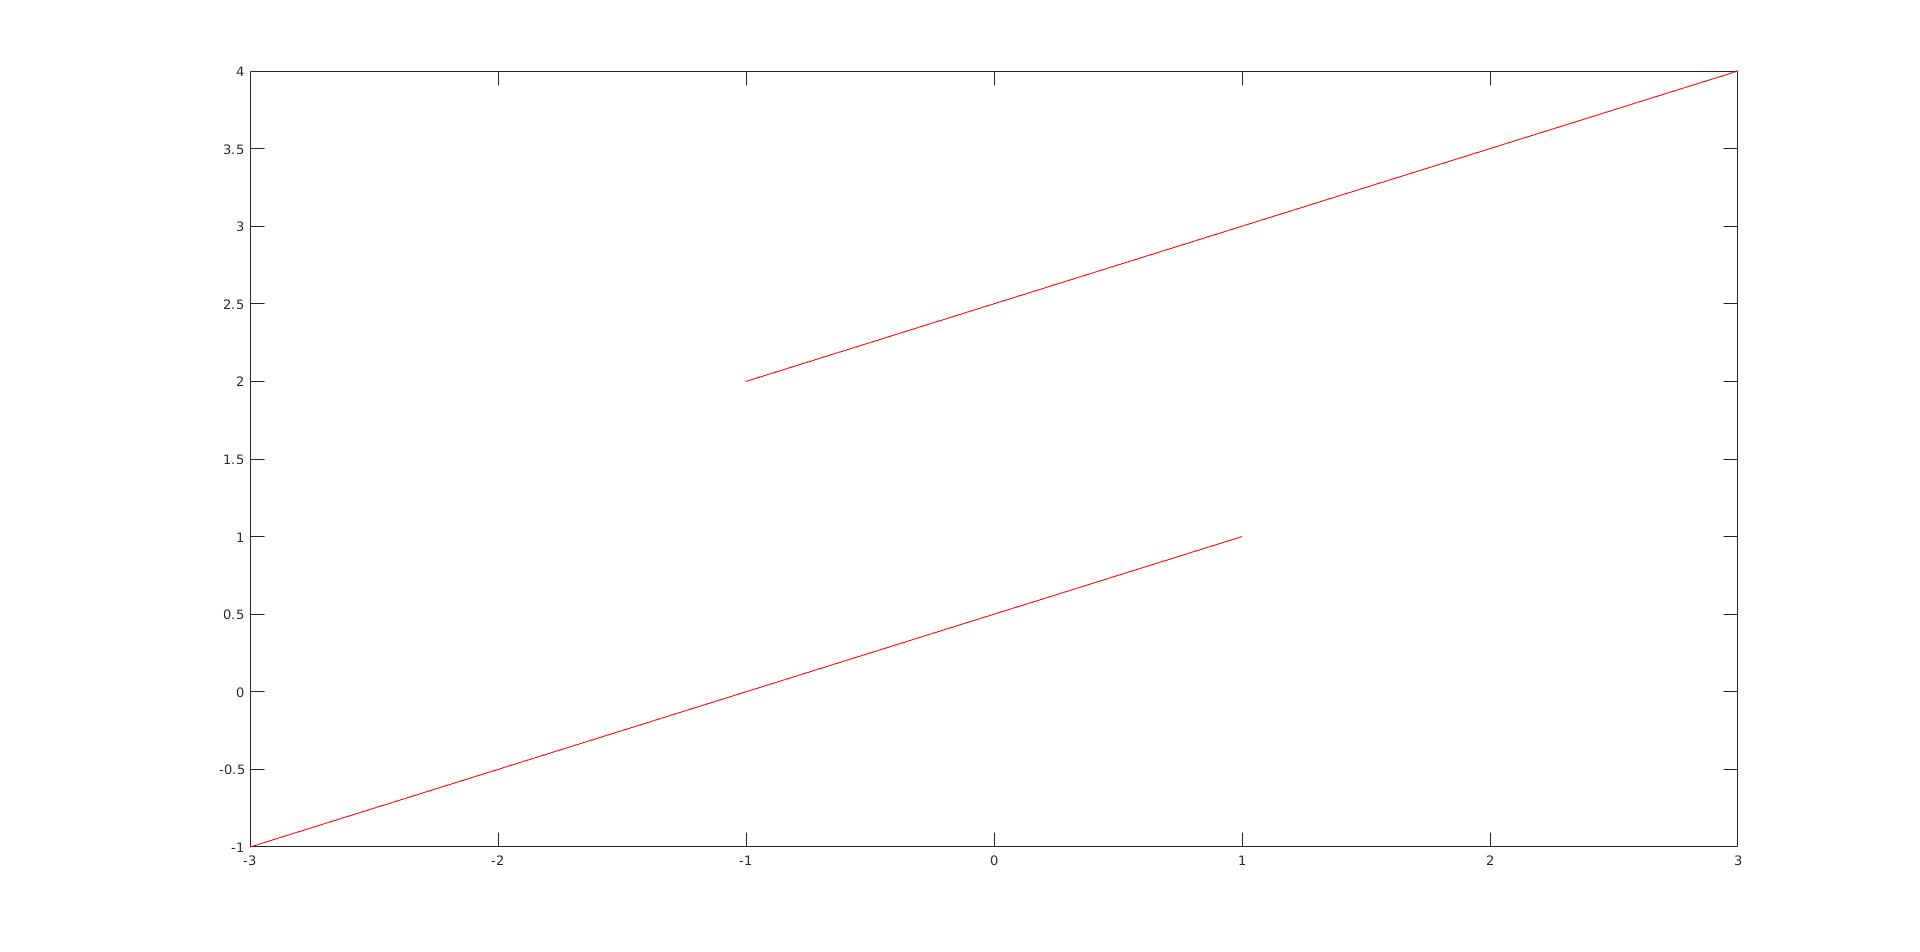
\includegraphics[scale=0.2]{figures/figure_01.jpg}
	\end{subfigure}%
\end{figure}

In homogeneous coordinate system, the $L_1$ is represented by:
\begin{equation}
l_1 \sim [1\ -2\ \ 5]^T
\end{equation}

and the $L_2$ is represented by:
\begin{equation}
l_2 \sim [1\ -2\ \ 1]^T
\end{equation}

In homogeneous coordinate system, given a point $X_1 \sim [x_1 \ \ y_1 \ \ z_1]^T$ which belongs to the line $l_1$. Other words,

\begin{equation}
	l_1^Tx_1 = 0
\end{equation}
 
 Similarly, we have other equation for $l_2$:
 
 \begin{equation}
 l_2^Tx_2 = 0
 \end{equation}
 
 where $X_2 \sim [x_2 \ \ y_2 \ \ z_2]^T$
 
 The intersection of the 2 lines is the roots for the following linear equation system:
 
 \begin{equation}
 	\systeme*{x_1 -2y_1 + 5z_1 = 0,x_1 -2y_1 + z_1 = 0}
 	\iff
 	\systeme*{x_1 = t, y_1 = \frac{t}{2}, z_1 = 0}
 \end{equation}
 
 Hence, for example $x_1 \sim [1 \ \frac{1}{2} \ 0]$ or $x_2 \sim [0 \ 0 \ 0]$ is represented our intersection point. We cannot interpret the result by diving the third component of $x_1$ because it is zero.
 
\end{homeworkProblem}

\begin{homeworkProblem}
\subsection{Crossing two points}
In the Cartesian coordinate system, given a line $L_1 = x -2y + 5 = 0$. Hence $L_1$ is presented by $l_1 \sim [1\ -2\ \ 5]^T$ in homogeneous coordinate system.

In homogeneous system, given 2 point $x_1 \sim [-1\ 2\ 1]^T$ and $x_2 \sim [3\ 4\ 1]^T$. We have:

\begin{equation}
	l_1^Tx_1 = [1\ -2\ \ 5]
	\begin{bmatrix}
	-1 \\
	 2 \\
	 1
	\end{bmatrix}
	= -1 -4 + 5 = 0
\end{equation}

Similarly for $x_2$
\begin{equation}
l_1^Tx_2 = [1\ -2\ \ 5]
\begin{bmatrix}
3 \\
4 \\
1
\end{bmatrix}
= 3 -8 + 5 = 0
\end{equation}

In the Cartesian coordinate, the points $x_1$ and $x_2$ belong to $L_1$. When they are converted to homogeneous coordinate, they are still in this line.

\end{homeworkProblem}
%----------------------------------------------------------------------------------------

%----------------------------------------------------------------------------------------
\begin{homeworkProblem}
    \subsection{2D Transformation in Matlab}
        \matlabscript{problem_3}{Demonstration of problem 3 in Matlab}

\begin{figure}[h]
	\centering
    \begin{subfigure}[h]{0.3\textwidth}
        \centering
        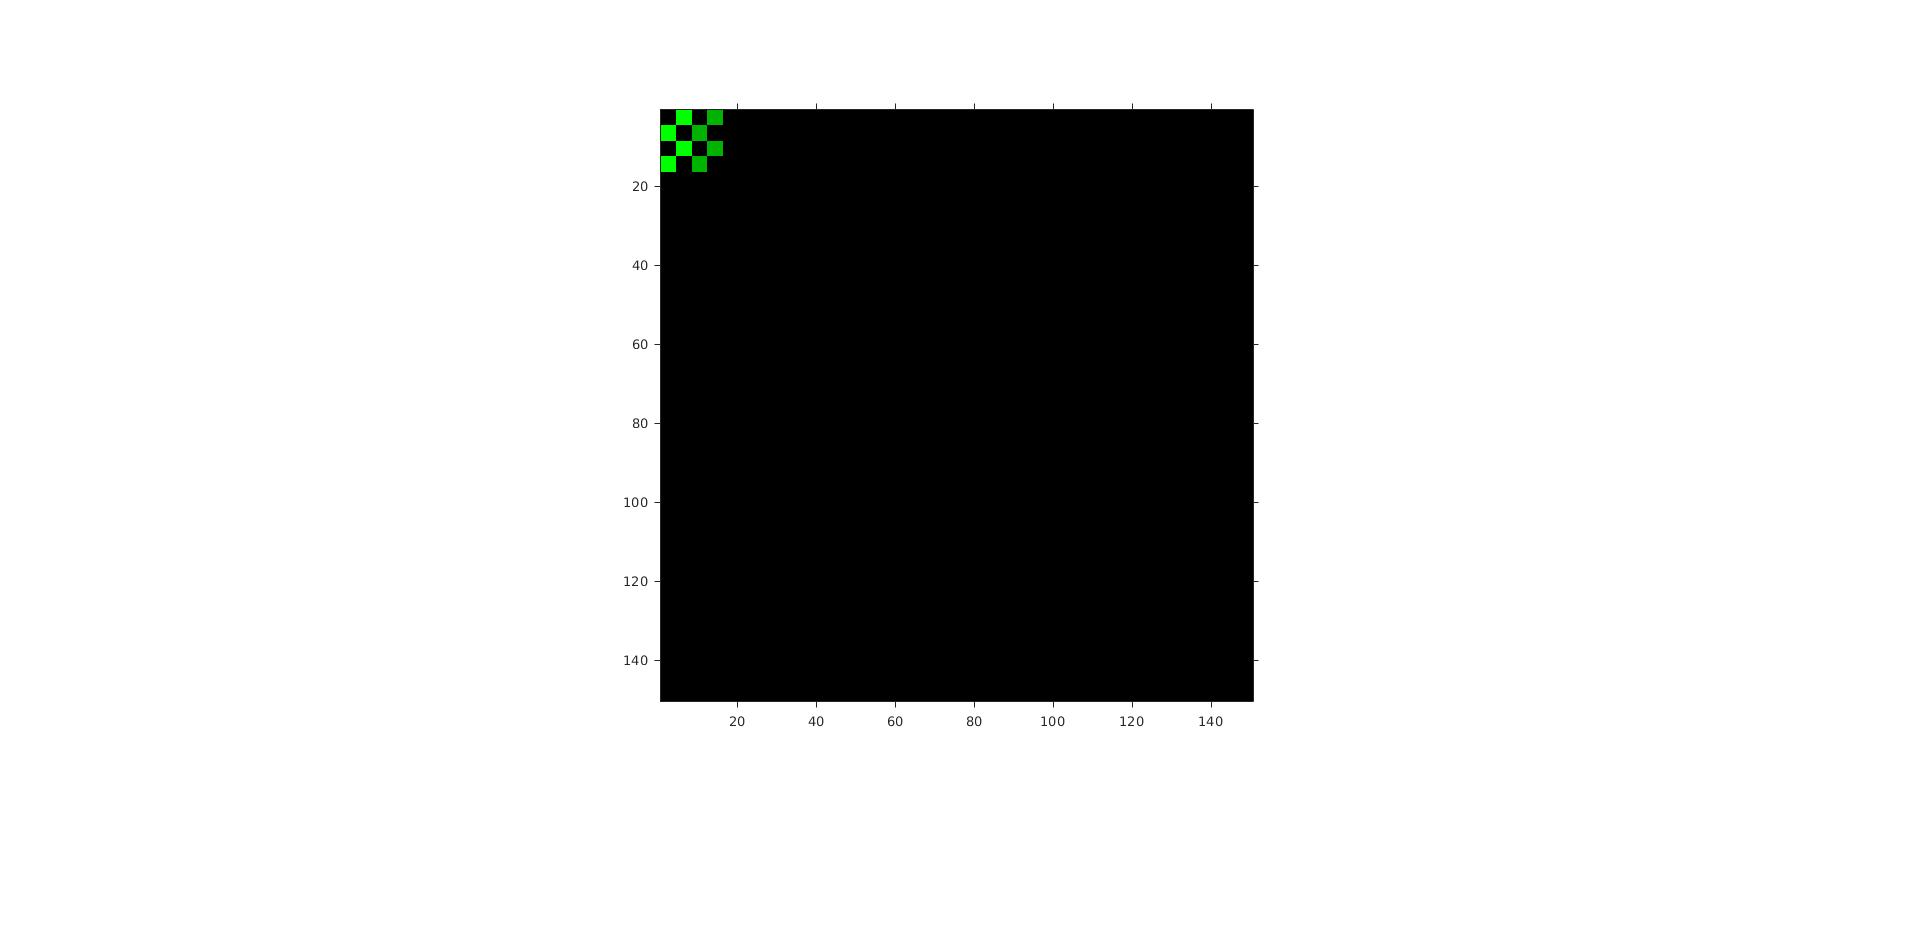
\includegraphics[scale=0.2]{figures/figure_02.jpg}
    \end{subfigure}%
\end{figure}

\begin{figure}[h]
	\centering
 \begin{subfigure}[h]{0.3\textwidth}
 	\centering
 	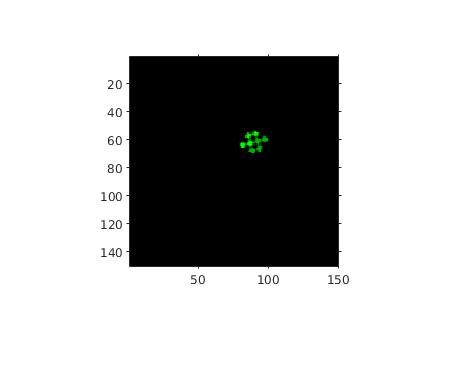
\includegraphics[scale=0.5]{figures/figure_03.jpg}
 \end{subfigure}%
\end{figure}

\end{homeworkProblem}
%----------------------------------------------------------------------------------------

\end{document}
